%\documentclass[12pt]{article}

\questionheader{ex:s1.5}


%%%%%%%%%%%%%%%%%%
\subsection*{\Conceptual}
%%%%%%%%%%%%%%%%%%
%%%%%%%%%%%%%%%%%%%
\begin{question}
What is wrong with the following exercise?

``Give an equation for the line passing through the point $(3,1,3)$ that is normal to the vectors $\llt 4,-6,2 \rgt$ and $\llt \frac13,-\frac12,\frac16 \rgt$."
\end{question}
\begin{hint}
What's fishy about those normal vectors? 
\end{hint}
\begin{answer}
There are infinitely many planes satisfying the condition described, but we're asked for ``the" line.

We need two normal directions to figure out the direction of a line in $\mathbb R^3$. Since the given normal vectors are parallel to each other, they really only specify \emph{one} normal direction. 
\end{answer}
\begin{solution}
Note $12\llt \frac13,-\frac12,\frac16 \rgt=\llt 4,-6,2 \rgt$. So, we actually only know one normal direction to the line we're supposed to be describing. That means there are actually \emph{infinitely many} lines satisfying the given conditions.

\begin{center}
\begin{tikzpicture}
\draw[thick,->] (0,0) node[vertex]{}--(0,2.5) node[above]{$\mathbf n$};
\clip (3,0) arc (0:360:3cm and 1cm);
\draw (-3,0)--(3,0);
\draw (-3,-1)--(3,1);
\draw (-3,1)--(3,-1);
\draw (-3,-2)--(3,2) (-3,2)--(3,-2) (3,-3)--(-3,-3) (1,2)--(-1,-2) (1,-2)--(-1,2);
\end{tikzpicture}
\end{center}

\end{solution}
%%%%%%%%%%%%%%%%%%%

%%%%%%%%%%%%%%%%%%%
\begin{question}
Find, if possible, four lines in 3d with
\begin{itemize}
\item
   no two of the lines parallel to each other and
\item
   no two of the lines intersecting.
\end{itemize}
\end{question}

\begin{hint}
The two lines $\llt x-x_0\,,\,y-y_0\,,\,z-z_0\rgt =t\vd$ and
$\llt x-x'_0\,,\,y-y'_0\,,\,z-z'_0\rgt =t\vd'$ are not parallel if
$\vd\times\vd'\ne\vZero$.
\end{hint}


\begin{answer}
There are infinitely many correct answers. One is
\begin{align*}
\llt x\,,\,x\,,\,z-1\rgt &= t\llt 1,0,0\rgt &
\llt x\,,\,x\,,\,z-2\rgt &= t\llt 0,1,0\rgt \\
\llt x\,,\,x\,,\,z-3\rgt &= t\llt 1,1,0\rgt &
\llt x\,,\,x\,,\,z-4\rgt &= t\llt 1,-1,0\rgt 
\end{align*}
 
\end{answer}
\begin{solution}
There are infinitely many correct answers. One is
\begin{align*}
L_1:\ \llt x\,,\,x\,,\,z-1\rgt &= t\llt 1,0,0\rgt &
L_2:\ \llt x\,,\,x\,,\,z-2\rgt &= t\llt 0,1,0\rgt \\
L_3:\ \llt x\,,\,x\,,\,z-3\rgt &= t\llt 1,1,0\rgt &
L_4:\ \llt x\,,\,x\,,\,z-4\rgt &= t\llt 1,-1,0\rgt 
\end{align*}
No two of the lines are parallel because
\begin{itemize}
\item
$L_1$ and $L_2$ are not parallel because
$\llt 1,0,0\rgt\times \llt 0,1,0\rgt=\llt 0,0,1\rgt\ne\vZero$.
\item
$L_1$ and $L_3$ are not parallel because
$\llt 1,0,0\rgt\times \llt 1,1,0\rgt=\llt 0,0,1\rgt\ne\vZero$.
\item
$L_1$ and $L_4$ are not parallel because
$\llt 1,0,0\rgt\times \llt 1,-1,0\rgt=\llt 0,0,-1\rgt\ne\vZero$.
\item
$L_2$ and $L_3$ are not parallel because
$\llt 0,1,0\rgt\times \llt 1,1,0\rgt=\llt 0,0,-1\rgt\ne\vZero$.
\item
$L_2$ and $L_4$ are not parallel because
$\llt 0,1,0\rgt\times \llt 1,-1,0\rgt=\llt 0,0,-1\rgt\ne\vZero$.
\item
$L_3$ and $L_4$ are not parallel because
$\llt 1,1,0\rgt\times \llt 1,-1,0\rgt=\llt 0,0,-2\rgt\ne\vZero$.
\end{itemize}
No two of the lines intersect because
\begin{itemize}
\item every point on $L_1$ has $z=1$ and
\item every point on $L_2$ has $z=2$ and
\item every point on $L_3$ has $z=3$ and
\item every point on $L_4$ has $z=4$.
\end{itemize}
\end{solution}


%%%%%%%%%%%%%%%%%%%%%%%%%%%%
%\Instructions{Questions~\ref{prob_s1.0first} through \ref{prob_s1.0last} provide practice with.}
%%%%%%%%%%%%%%%%%%%%

%%%%%%%%%%%%%%%%%%
\subsection*{\Procedural}
%%%%%%%%%%%%%%%%%%

%%%%%%%%%%%%%%%%%%%%%%%%%%%%%%%%%%%%
\begin{question}
Find a vector parametric equation for the line of intersection
of the given planes.
\begin{enumerate}[(a)]
\item $x-2z=3$ and $y+\half z=5$
\item $2x-y-2z=-3$ and $4x-3y-3 z=-5$
\end{enumerate}
\end{question}

\begin{hint}
Review Example \eref{CLP200}{eg line equations} in the CLP-3 text.
\end{hint}

\begin{answer}
(a) $\llt x,y,z\rgt =  \llt 3,5,0\rgt+\llt 2,-\half,1\rgt t$

(b) $\llt x,y,z\rgt =  \llt -2,-1,0\rgt +\llt \frac{3}{2},1,1\rgt t$
\end{answer}

\begin{solution}
(a) The point $(x,y,z)$ obeys both $x-2z=3$ and $y+\half z=5$
if and only if $\llt x,y,z\rgt = \llt 3+2z, 5-\half z, z\rgt 
                  = \llt 3,5,0\rgt+\llt 2,-\half,1\rgt z$.
So, introducing a new variable $t$ obeying $t=z$, we get the vector 
parametric equation $\llt x,y,z\rgt =  \llt 3,5,0\rgt+\llt 2,-\half,1\rgt t$.

(b) The point $(x,y,z)$ obeys 
\begin{align*}
\left\{\Atop{2x-y-2z=-3}{4x-3y-3 z=-5} \right\}
&\iff \left\{\Atop{2x-y=2z-3}{4x-3y=3 z-5} \right\}
\iff\left\{\Atop{4x-2y=4z-6}{4x-3y=3 z-5} \right\}\\
\noalign{\vskip0.1in}
&\iff\left\{\Atop{4x-2y=4z-6}{y=z-1} \right\}
\end{align*}
Hence the point $(x,y,z)$ is on the line if and only if 
$\llt x,y,z\rgt = \llt \frac{1}{4}(2y+4z-6), z-1, z\rgt=
\llt \frac{3}{2}z-2, z-1, z\rgt = \llt -2,-1,0\rgt+\llt \frac{3}{2},1,1\rgt z$.
So, introducing a new variable $t$ obeying $t=z$, we get the vector 
parametric equation $\llt x,y,z\rgt =  \llt -2,-1,0\rgt
        +\llt \frac{3}{2},1,1\rgt t$.
\end{solution}

%%%%%%%%%%%%%%%%%%%%%%%%%%%%%%%%%%%%
\begin{question}
Determine a vector equation for the line of intersection
of the planes
\begin{enumerate}[(a)]
\item $x+y+z=3$ and $x+2y+3z=7$
\item $x+y+z=3$ and $2x+2y+2z=7$
\end{enumerate}
\end{question}

\begin{hint}
Review Example \eref{CLP200}{eg line equations} in the CLP-3 text.
\end{hint}

\begin{answer}
(a) $\llt x,y,z\rgt=\llt -1,4,0\rgt+t\llt 1,-2,1\rgt $

(b) The two planes are parallel and \emph{do not intersect}.

\end{answer}

\begin{solution}
(a) The normals to the two planes are $\llt 1,1,1\rgt $ and $\llt 1,2,3\rgt $
respectively. The line of intersection must have direction perpendicular
to both of these normals. Its direction vector is 
\begin{equation*}
\llt 1,1,1\rgt \times\llt 1,2,3\rgt 
=\det\left[\begin{matrix} \hi &\hj &\hk \\ 1&1&1 \\ 1&2&3 \end{matrix}\right]
=\llt 1,-2,1\rgt 
\end{equation*}
Substituting $z=0$ into the equations of the two planes and solving
\begin{align*}
\left\{\Atop{x+y=3}{x+2y=7} \right\}
&\iff \left\{\Atop{x=3-y}{x+2y=7} \right\}
\iff\left\{\Atop{x=3-y}{3-y+2y=7} \right\}
\end{align*}
we see that $z=0,\ y=4, x=-1$ lies on both planes. The line of
intersection is $\llt x,y,z\rgt=\llt -1,4,0\rgt+t\llt 1,-2,1\rgt $. 
This can be checked by verifying that,  for all values of $t$, 
$\llt x,y,z\rgt=\llt -1,4,0\rgt+t\llt 1,-2,1\rgt $ satisfies both 
$x+y+z=3$ and $x+2y+3z=7$.

(b) The equation $x+y+z=3$ is equivalent to $2x+2y+2z=6$.
So the two equations $x+y+z=3$ and $2x+2y+2z=7$ are mutually
contradictory. They have no solution. The two planes are parallel and
\emph{do not intersect}.
\end{solution}

%%%%%%%%%%%%%%%%%%%%%%%%%%%%%%%%%%%%
\begin{question}
In each case, determine whether or not the given pair
of lines intersect. Also find all planes containing the pair of lines.
\begin{enumerate}[(a)]
\item $\llt x,y,z\rgt = \llt -3,2,4\rgt+t\llt -4,2,1\rgt$ and 
      $\llt x,y,z\rgt = \llt 2,1,2\rgt+t\llt 1,1,-1\rgt$
\item $\llt x,y,z\rgt = \llt -3,2,4\rgt+t\llt -4,2,1\rgt$ and 
      $\llt x,y,z\rgt = \llt 2,1,-1\rgt+t\llt 1,1,-1\rgt$
\item $\llt x,y,z\rgt = \llt -3,2,4\rgt+t\llt -2,-2,2\rgt$ and 
      $\llt x,y,z\rgt = \llt 2,1,-1\rgt+t\llt 1,1,-1\rgt$
\item $\llt x,y,z\rgt = \llt 3,2,-2\rgt+t\llt -2,-2,2\rgt$ and 
      $\llt x,y,z\rgt = \llt 2,1,-1\rgt+t\llt 1,1,-1\rgt$
\end{enumerate}
\end{question}

%\begin{hint}
%\end{hint}

\begin{answer}
(a) $(1,0,3)$ lies on both lines.
     $x+y+2z=7$ is the only plane containing both lines.

(b) The two lines do not intersect. No plane contains the two lines.

(c) The two lines do not intersect.
     $x+z=1$ is the only plane containing both lines.

(d) The two lines are identical.
    For arbitrary $a$ and $b$ (not both zero) the plane $ax+by+(a+b)z=a$
    contains both lines.
\end{answer}

\begin{solution}
(a) Note that the value of the parameter $t$ in the 
equation $\llt x,y,z\rgt = \llt -3,2,4\rgt+t\llt -4,2,1\rgt$ 
need not have the same value as the parameter $t$ in the 
equation $\llt x,y,z\rgt = \llt 2,1,2\rgt+t\llt 1,1,-1\rgt$. So it is 
much safer to change the name of the parameter in the first equation 
from $t$ to $s$. In order for a point $(x,y,z)$ to lie on both 
lines we need
\begin{equation*}
\llt -3,2,4\rgt+s\llt -4,2,1\rgt = \llt 2,1,2\rgt+t\llt 1,1,-1\rgt
\end{equation*}
or equivalently, writing out the three component equations and moving
all $s$'s and $t$'s to the left and constants to the right,
\begin{align*}
-4s -t &= 5\\
2s -t &= -1\\
s +t &= -2
\end{align*}
Adding the last two equations together gives $3s=-3$ or $s=-1$. Substituting
this into the last equation gives $t=-1$. Note that $s=t=-1$ does indeed
satisfy all three equations so that 
 $\llt x,y,z\rgt=\llt -3,2,4\rgt-\llt -4,2,1\rgt=\llt 1,0,3\rgt$
lies on both lines. Any plane that contains the two lines must be parallel
to both direction vectors $\llt -4,2,1\rgt$ and $\llt 1,1,-1\rgt$. So 
its normal vector must be perpendicular to them, i.e. must be parallel to 
$\llt -4,2,1\rgt\times\llt 1,1,-1\rgt=\llt -3,-3,-6\rgt=-3\llt 1,1,2\rgt$. 
The plane must contain $(1,0,3)$ and be perpendicular to $\llt 1,1,2\rgt$. 
Its equation is $\llt 1,1,2\rgt\cdot\llt x-1,y,z-3\rgt=0$ or $x+y+2z=7$. 
This can be checked by verifying that $\llt -3,2,4\rgt+s\llt -4,2,1\rgt$ and 
$\llt 2,1,2\rgt+t\llt 1,1,-1\rgt$ obey
$x+y+2z=7$ for all $s$ and $t$ respectively. 

(b) In order for a point $(x,y,z)$ to lie on both lines we need
\begin{equation*}
\llt -3,2,4\rgt+s\llt -4,2,1\rgt = \llt 2,1,-1\rgt+t\llt 1,1,-1\rgt
\end{equation*}
or equivalently, writing out the three component equations and moving
all $s$'s and $t$'s to the left and constants to the right,
\begin{align*}
-4s -t &= 5\\
2s -t &= -1\\
s +t &= -5
\end{align*}
Adding the last two equations together gives $3s=-6$ or $s=-2$. Substituting
this into the last equation gives $t=-3$. However, substituting 
$s=-2,\ t=-3$ into the first equation gives $11=5$, which is impossible. The
two lines \emph{do not intersect}. In order for two lines to lie
in a common plane and not intersect, they must be parallel. So, in this
case \emph{no plane contains the two lines}.

(c) In order for a point $(x,y,z)$ to lie on both lines we need
\begin{equation*}
\llt -3,2,4\rgt+s\llt -2,-2,2\rgt = \llt 2,1,-1\rgt+t\llt 1,1,-1\rgt
\end{equation*}
or equivalently, writing out the three component equations and moving
all $s$'s and $t$'s to the left and constants to the right,
\begin{align*}
-2s -t &= 5\\
-2s -t &= -1\\
2s +t &= -5
\end{align*}
The first two equations are obviously contradictory. The
two lines \emph{do not intersect}. Any plane containing the two lines 
must be parallel to $\llt 1,1,-1\rgt$ (and hence automatically parallel
to $\llt -2,-2,2\rgt=-2\llt 1,1,-1\rgt$) and must also be parallel to the vector
from the point $(-3,2,4)$, which lies on the first line, to the point
$(2,1,-1)$, which lies on the second. The vector is $\llt 5,-1,-5\rgt$. 
Hence the normal to the plane is 
$\llt 5,-1,-5\rgt\times\llt 1,1,-1\rgt=\llt 6,0,6\rgt=6\llt 1,0,1\rgt$.
The plane perpendicular to $\llt 1,0,1\rgt$ containing $(2,1,-1)$ is
$\llt 1,0,1\rgt\cdot\llt x-2,y-1,z+1\rgt=0$ or $x+z=1$.

(d) Again the two lines are parallel, since 
$\llt -2,-2,2\rgt=-2\llt 1,1,-1\rgt$.
Furthermore the point 
$\llt 3,2,-2\rgt=\llt 3,2,-2\rgt+0\llt -2,-2,2\rgt
       =\llt 2,1,-1\rgt+1\llt 1,1,-1\rgt$
lies on both lines. So the two lines not only \emph{intersect} but
are identical. Any plane that contains the point $(3,2,-2)$ and is parallel
to $\llt 1,1,-1\rgt$ contains both lines. In general, the plane $ax+by+cz=d$
contains $(3,2,-2)$ if and only if $d=3a+2b-2c$ and is parallel to 
$\llt 1,1,-1\rgt$ if and only if $\llt a,b,c\rgt\cdot\llt 1,1,-1\rgt=a+b-c=0$. So, for arbitrary $a$ and $b$ (not both zero) $ax+by+(a+b)z=a$ works.
\end{solution}




%%%%%%%%%%%%%%%%%%%%%%%%%%%%%%%%
\begin{question}
Find the equation of the line through $(2,-1,-1)$ and parallel
to each of the two planes $x+y=0$ and $x-y+2z=0$. Express the equations
of the line in vector and scalar parametric forms and in symmetric form.
\end{question}

%\begin{hint}
%
%\end{hint}

\begin{answer}
vector parametric equation:\ \ \ $\llt x-2,y+1,z+1\rgt= t\llt 1,-1,-1\rgt$

scalar parametric equation:\ \ \ $x=2+t$,  $y=-1-t$,  $z=-1-t$

symmetric equation:\ \ \ $x-2=-y-1=-z-1$
\end{answer}

\begin{solution}
First observe that
\begin{itemize}
\item
$\llt 1,1,0\rgt$ is perpendicular to $x+y=0$  and hence to the line, and
\item
$\llt 1,-1,2\rgt$ is perpendicular to $x-y+2z=0$  and hence to the line.
\end{itemize}
Consequently
\begin{align*}
\llt 1\,,\,1\,,\,0\rgt \times \llt 1\,,\,-1\,,\,2\rgt
    =\det\left[\begin{matrix}
            \hi  &  \hj  &  \hk \\
            1    &   1   &   0 \\
            1    &  -1   &   2 
            \end{matrix}\right]
=\llt 2 \,,\, -2 \,,\, -2 \rgt
\end{align*}
is perpendicular to both $\llt 1,1,0\rgt$ and $\llt 1,-1,2\rgt$.
So $\frac{1}{2}\llt 2 \,,\, -2 \,,\, -2 \rgt=\llt 1,-1,-1\rgt\>$
is also perpendicular to both $\llt 1,1,0\rgt$ and $\llt 1,-1,2\rgt$
and hence is parallel to the line. As the point $(2,-1,-1)$ is on the line,
the vector  equation of the line is
\begin{equation*}
\llt x-2,y+1,z+1\rgt= t\llt 1,-1,-1\rgt
\end{equation*}
The scalar parametric equations for the line are
\begin{align*}
x-2=t,\ 
y+1=-t,\ 
z+1=-t
\hskip .25 in\hbox{or}\hskip .25 in
x=2+t,\ 
y=-1-t,\ 
z=-1-t
\end{align*}
The symmetric equations for the line are
\begin{align*}
(t=)\frac{x-2}{1}=\frac{y+1}{-1}=\frac{z+1}{-1}
\hskip .25 in\hbox{or}\hskip .25 in
x-2=-y-1=-z-1
\end{align*}


\end{solution}

%%%%%%%%%%%%%%%%%%%%%%%%%%%%%%%%
\begin{question}[M200 2011A] %1a
Let  $L$ be the line given by the equations $x + y = 1$ and
$x + 2y + z = 3$.
Write a vector parametric equation for $L$.
\end{question}

\begin{hint}
Review Example \eref{CLP200}{eg line equations} in the CLP-3 text.
\end{hint}

\begin{answer}
$\llt x,y,z\rgt = \llt 1,0,2\rgt +t\llt-1,1,-1 \rgt$
\end{answer}

\begin{solution}
Let's parametrize $L$ using $y$, renamed to $t$, as the parameter.
Then $y=t$, so that 
\begin{equation*}
x+y=1
\implies x+t=1
\implies x=1-t
\end{equation*}
and
\begin{equation*}
x+2y+z=3
\implies
1-t + 2t +z =3
\implies z = 2-t
\end{equation*}
and
\begin{equation*}
\llt x,y,z\rgt = \llt 1,0,2\rgt +t\llt-1,1,-1 \rgt
\end{equation*}
is a vector parametric equation for $L$.
\end{solution}

%%%%%%%%%%%%%%%%%%%%%%%%%%%%%%%%
\begin{question}
\begin{enumerate}[(a)]
\item
Find a vector parametric equation for the line
$x+2y+3z=11,\ x-2y+z=-1$. 
\item
Find the distance from $(1,0,1)$ to the line
$x+2y+3z=11,\ x-2y+z=-1$. 
\end{enumerate}
\end{question}

\begin{hint}
Review Example \eref{CLP200}{eg:VPdistance-point-line} in the CLP-3 text.
\end{hint}

\begin{answer}
(a) $\llt x,y,z\rgt=\llt 5,3,0\rgt+t\llt 4,1,-2\rgt =\llt 5+4t,3+t,-2t\rgt$.
\qquad
(b) $\sqrt{5}$
\end{answer}

\begin{solution} (a)
The normal vectors to the two given planes are 
$\llt 1,2,3\rgt $ and $\llt 1,-2,1\rgt $ respectively. 
Since the line is to be contained in both planes, its direction vector 
must be perpendicular to both $\llt 1,2,3\rgt $ and $\llt 1,-2,1\rgt $, 
and hence must be parallel to 
\begin{equation*}
\llt 1,2,3\rgt \times\llt 1,-2,1\rgt 
=\det\left[\begin{matrix}
           \hi & \hj & \hk \\
           1  &  2  &  3 \\
           1  &  -2  & 1
  \end{matrix}\right]
=\llt 8, 2,-4\rgt
\end{equation*} 
or to $\llt 4,1,-2\rgt $. Setting $z=0$ in $x+2y+3z=11,\ x-2y+z=-1$ and
solving 
\begin{align*}
\left\{\Atop{x+2y=11}{x-2y=-1} \right\}
\iff \left\{\Atop{2y=11-x}{x-2y=-1} \right\}
\iff \left\{\Atop{2y=11-x}{x-(11-x)=-1} \right\}
\iff \left\{\Atop{2y=11-x}{2x=10} \right\}
\end{align*}
we see that $(5,3,0)$ is on the line. So
the vector parametric equation of the line is 
$\llt x,y,z\rgt=\llt 5,3,0\rgt+t\llt 4,1,-2\rgt =\llt 5+4t,3+t,-2t\rgt$.


\noindent (b) 
The vector from $(1,0,1)$ to the point $(5+4t,3+t,-2t)$ on the line
is $\llt 4+4t,3+t,-1-2t\rgt$. In order for $(5+4t,3+t,-2t)$ to be the point 
of the line closest to $(1,0,1)$, the vector $\llt 4+4t,3+t,-1-2t\rgt$ 
joining those two points must be perpendicular to the direction vector 
$\llt 4,1,-2\rgt $ of the line. (See Example \eref{CLP200}{eg:VPdistance-point-line}  in the CLP-3 text.)
This is the case when
\begin{equation*}
\llt 4,1,-2\rgt \cdot \llt 4+4t,3+t,-1-2t\rgt =0\quad\text{or}\quad
16+16t+3+t+2+4t=0\quad\text{or}\quad t=-1
\end{equation*}
The point on the line nearest $(1,0,1)$ is thus 
$(5+4t,3+t,-2t)\Big|_{t=-1}=(5-4,3-1,2)=(1,2,2)$. The distance
from the point to the line is the length of the vector from
$(1,0,1)$ to the point on the line nearest $(1,0,1)$. That vector is 
$\llt 1,2,2\rgt -\llt 1,0,1\rgt =\llt 0,2,1\rgt$. So the distance is 
$|\llt 0,2,1\rgt|=\sqrt{5}$.
\end{solution}

%%%%%%%%%%%%%%%%%%%%%%%%%%%%%%%%
\begin{question}
Let $L_1$ be the line passing through $(1,-2,-5)$ in the direction of 
$\vd_1=\llt 2,3,2\rgt$. 
Let $L_2$ be the line passing through $(-3,4,-1)$ in the direction 
$\vd_2=\llt 5,2,4\rgt$.
\begin{enumerate}[(a)]
\item
Find the equation of the plane $P$ that contains $L_1$
and is parallel to $L_2$.
\item
Find the distance from $L_2$ to $P$.
\end{enumerate}
\end{question}

\begin{hint}
Review Example \eref{CLP200}{eg:VPdistance-point-plane} in the CLP-3 text.
\end{hint}

\begin{answer}
(a) $8x+2y-11z=59$\qquad
(b) $\frac{64}{\sqrt{189}} \approx 4.655$
\end{answer}

\begin{solution}
(a) The plane $P$ must be parallel to both $\llt 2,3,2\rgt $ (since it 
contains $L_1$) and $\llt 5,2,4\rgt $ (since it is parallel to $L_2$).
Hence 
\begin{equation*}
\llt 2,3,2\rgt \times \llt 5,2,4\rgt 
=\det\left[\begin{matrix}
           \hi & \hj & \hk \\
           2  &  3  & 2 \\
           5  &  2  & 4
  \end{matrix}\right]
=\llt 8,2,-11\rgt 
\end{equation*}
is normal to $P$. As the point $(1,-2,-5)$ is on $P$, the equation
of $P$ is
\begin{equation*}
\llt 8,2,-11\rgt \cdot\llt x-1,y+2,z+5\rgt =0\qquad \text{or}\qquad 8x+2y-11z=59
\end{equation*}

(b) As $L_2$ is parallel to $P$, the distance from $L_2$ to $P$ is the
same as the distance from any one point of $L_2$, for example $(-3,4,-1)$,
to $P$. As $(1,-2,-5)$ is a point on $P$, the vector 
$\llt 1,-2,-5\rgt-\llt -3, 4,-1\rgt =\llt 4,-6,-4\rgt $ has its head on $P$ 
and tail at $(-3,4,-1)$ on $L_2$. 
The distance from $L_2$ to $P$ is the length of the projection of the vector $\llt 4,-6,-4\rgt $ on the normal to $P$. (See Example \eref{CLP200}{eg:VPdistance-point-plane-bis} in the CLP-3 text.) This is 
\begin{equation*}
\left|\text{proj}_{\llt 8,2,-11\rgt}\llt 4,-6,-4\rgt\right|
=\frac{|\llt 4,-6,-4\rgt \cdot\llt 8,2,-11\rgt|} {|\llt 8,2,-11\rgt|}
=\frac{64}{\sqrt{189}}
\approx4.655
\end{equation*}
\end{solution}


%%%%%%%%%%%%%%%%%%%%%%%%%%%%%%%%
\begin{question}[M200 2012a] %1
Let $L$ be a line which is parallel to the plane $2x + y  - z = 5$ and 
perpendicular to the line $x = 3 - t$, $y = 1 - 2t$ and $z = 3t$.
\begin{enumerate}[(a)]
\item
Find a vector parallel to the line $L$.
\item
Find parametric equations for the line $L$ if $L$ passes through a point 
$Q(a, b, c)$
where $a < 0$, $b > 0$, $c > 0$, and the distances from $Q$ to the $xy$--plane, 
the $xz$--plane and the $yz$--plane are $2$, $3$ and $4$ respectively.
\end{enumerate}
\end{question}

%\begin{hint}
%
%\end{hint}

\begin{answer}
(a) Any nonzero constant times $\llt 1 \,,\, -5 \,,\, -3 \rgt$.\qquad
(b) $x = -4 + t$, 
    $y = 3 - 5t$,
    $z = 2 - 3t$
\end{answer}

\begin{solution}
(a) The line $L$ must be perpendicular both to 
        $\llt 2\,,\,1\,,\,-1\rgt$, which is a normal vector 
        for the plane $2x + y  - z = 5$,
and to
        $\llt -1\,,\,-2\,,\,3\rgt$, which is a direction vector for
the line $x = 3 - t$, $y = 1 - 2t$ and $z = 3t$.
Any such vector must be a nonzero constant times
\begin{align*}
\llt 2\,,\,1\,,\,-1\rgt \times \llt -1\,,\,-2\,,\,3\rgt
    =\det\left[\begin{matrix}
            \hi  &  \hj  &  \hk \\
            2    &   1   &    -1 \\
           -1    &  -2   &   3 
            \end{matrix}\right]
=\llt 1 \,,\, -5 \,,\, -3 \rgt
\end{align*}

(b) For the point $Q(a, b, c)$
\begin{itemize}
\item
to be a distance $2$ from the $xy$--plane, it is necessary that $|c|=2$,
and
\item
to be a distance $3$ from the $xz$--plane, it is necessary that $|b|=3$,
and
\item
to be a distance $4$ from the $yz$--plane, it is necessary that $|a|=4$.
\end{itemize}
As $a < 0$, $b > 0$, $c > 0$, the point $Q$ is $(-4, 3, 2)$ and the line $L$
is
\begin{equation*}
x = -4 + t \qquad
y = 3 - 5t \qquad
z = 2 - 3t 
\end{equation*}
\end{solution}

%%%%%%%%%%%%%%%%%%%%%%%%%%%%%%%%
\begin{question}[M200 2012D] %1
Let $L$ be the line of intersection of the planes $x + y + z = 6$ and 
$x - y + 2z = 0$.
\begin{enumerate}[(a)]
\item
Find the points in which the line $L$ intersects the coordinate planes.
\item
Find parametric equations for the line through the point $(10, 11, 13)$ 
that is perpendicular to the line $L$ and parallel to the plane $y = z$.
\end{enumerate}
\end{question}

%\begin{hint}
%
%\end{hint}

\begin{answer}
(a) $(3,3,0)$,  $(12,0,-6)$, $(0,4,2)$ \qquad
(b) $x=10+t$, $y=11+t$, $z=13+t$.
\end{answer}

\begin{solution}
(a)
The line $L$ intersects the $xy$--plane when 
$x + y + z = 6$,
$x - y + 2z = 0$,
and $z=0$. When $z=0$ the equations of $L$ reduce to 
$x + y = 6$,
$x - y = 0$.
So the intersection point is $(3,3,0)$.

The line $L$ intersects the $xz$--plane when 
$x + y + z = 6$,
$x - y + 2z = 0$,
and $y=0$. When $y=0$ the equations of $L$ reduce to 
$x + z = 6$,
$x +2z = 0$.
Substituting $x=-2z$ into $x+z=6$ gives $-z=6$.
So the intersection point is $(12,0,-6)$.

The line $L$ intersects the $yz$--plane when 
$x + y + z = 6$,
$x - y + 2z = 0$,
and $x=0$. When $x=0$ the equations of $L$ reduce to 
$y + z = 6$,
$-y +2z = 0$.
Substituting $y=2z$ into $y+z=6$ gives $3z=6$.
So the intersection point is $(0,4,2)$.

(b)
Our main job is to find a direction vector $\vd$ for the line.
\begin{itemize}
\item
Since the line is to be parallel to $y=z$, $\vd$ must be perpendicular
to the normal vector for $y=z$, which is $\llt 0,1,-1\rgt$. 
\item
$\vd$ must also be perpendicular to $L$. For a point $(x,y,z)$ to be on $L$
it must obey $x+y = 6-z$ and $x-y =-2z$. Adding these two equations
gives $2x=6-3z$ and subtracting the second equation from the first
gives $2y= 6+z$. So for a point $(x,y,z)$ to be on $L$ it must obey 
$x=3-\frac{3z}{2}$, $y=3+\frac{z}{2}$. The point on $L$ with $z=0$
is $(3,3,0)$ and the point on $L$ with $z=2$ is $(0,4,2)$. So
 $\llt 0-3,4-3,2-0 \rgt=\llt -3,1,2 \rgt$ is a direction vector for $L$.
\end{itemize}
So $\vd$ must be perpendicular to both $\llt 0,1,-1\rgt$
and $\llt -3,1,2 \rgt$ and so must be a nonzero constant times
\begin{align*}
\llt 0,1,-1\rgt \times \llt -3,1,2 \rgt
    =\det\left[\begin{matrix}
            \hi  &  \hj  &  \hk \\
            0    &   1   &   -1 \\
            -3    &   1   &    2 
            \end{matrix}\right]
=\llt 3 \,,\, 3 \,,\, 3 \rgt
\end{align*}
We choose $\vd=\frac{1}{3}\llt 3 \,,\, 3 \,,\, 3 \rgt=\llt 1\,,\,1\,,\,1 \rgt$.
So 
\begin{equation*}
\llt x,y,z\rgt = \llt 10,11,13\rgt + t \llt 1\,,\,1\,,\,1 \rgt
\end{equation*}
is a vector parametric equation for the line. We can also write this as
$x=10+t$, $y=11+t$, $z=13+t$.
\end{solution}

%%%%%%%%%%%%%%%%%%%%%%%%%%%%%%%%
\begin{question}[M200 2013D] %1a
The line $L$ has vector parametric equation 
$\vr(t) = (2 + 3t)\hi + 4t\hj - \hk$.
\begin{enumerate}[(a)]
\item
Write the symmetric equations for $L$.
\item
Let $\alpha$ be the angle between the line $L$ and the plane given 
by the equation $x - y + 2z = 0$. Find $\alpha$.
\end{enumerate}
\end{question}

\begin{hint}
Review the properties of the dot product in 
Theorem \eref{CLP200}{thm:dotPppties} of the CLP-3 text.
\end{hint}

\begin{answer}
(a)  $\frac{x-2}{3}=\frac{y}{4}\qquad z=-1$

(b)  $\al =\frac{\pi}{2}-\arccos\frac{1}{5\sqrt{6}}
             \approx 0.08\,\text{radians}$
\end{answer}

\begin{solution}
(a)  Since
\begin{alignat*}{3}
x&=2+3t &&\implies t=\frac{x-2}{3} \\
y&=4t   &&\implies t=\frac{y}{4}
\end{alignat*}
we have
\begin{equation*}
\frac{x-2}{3}=\frac{y}{4}\qquad z=-1
\end{equation*}

(b) The direction vector for the line 
   $\vr(t) = 2\,\hi-\hk +t(3\,\hi+4\,\hj)$
  is $\vd=3\,\hi+4\,\hj$. A normal vector for the plane $x-y+2z=0$ is 
   $\vn=\pm\big(\hi-\hj+2\,\hk\big)$. The angle $\theta$ between $\vd$ 
   and $\vn$ obeys
\begin{align*}
\cos\theta =\frac{\vd\cdot\vn}{|\vd|\,|\vn|}
           =\frac{1}{5\sqrt{6}}
\implies \theta =\arccos\frac{1}{5\sqrt{6}}\approx 1.49\,\text{radians}
\end{align*}
(We picked $\vn=-\hi+\hj-2\hk$ to make $0\le\theta\le\frac{\pi}{2}$.)
Then the angle between $\vd$ and the plane is
\begin{equation*}
\al =\frac{\pi}{2}-\arccos\frac{1}{5\sqrt{6}}\approx 0.08\,\text{radians}
\end{equation*}

\begin{center}
     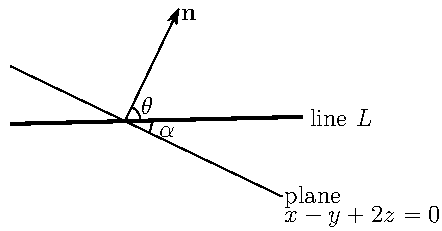
\includegraphics{OE13D_1.pdf}
\end{center}


\end{solution}

%%%%%%%%%%%%%%%%%%%%%%%%%%%%%%%%
\begin{question}[M200 2015D] %1b
Find the parametric equation for the line of intersection of the 
planes
\begin{equation*}
x + y + z = 11\qquad \text{and}\qquad x - y - z = 13.
\end{equation*}
\end{question}

%\begin{hint}
%
%\end{hint}

\begin{answer}
$(x,y,z) = \big(12\,,\,-1-t\,,\,t\big)$
\end{answer}

\begin{solution}
Let's use $z$ as the parameter and call it $t$. Then $z=t$
and
\begin{align*}
x+y&=11-t \\
x-y&=13+t
\end{align*}
Adding the two equations gives $2x=24$ and subtracting the
second equation from the first gives $2y=-2-2t$. So
\begin{equation*}
(x,y,z) = \big(12\,,\,-1-t\,,\,t\big)
\end{equation*}
\end{solution}

%%%%%%%%%%%%%%%%%%%%%%%%%%%%%%%%
\begin{question}[M200 2000A] %1
\begin{enumerate}[(a)]
\item
Find a point on the y-axis equidistant from 
                $(2, 5, -3)$ and $(-3, 6, 1)$. 

\item  
Find the equation of the plane containing the point 
           $(1, 3, 1)$ and the line $\vr(t) = t\,\hi + t\,\hj + (t + 2)\,\hk$.
\end{enumerate}
\end{question}

%\begin{hint}
%
%\end{hint}

\begin{answer}
(a) $(0,4,0)$\qquad
(b) $2x-y-z=-2$
\end{answer}

\begin{solution}
(a) 
The point $(0,y,0)$, on the $y$--axis, is equidistant from 
                $(2, 5, -3)$ and $(-3, 6, 1)$ if and only if
\begin{align*}
&\big|\llt 2, 5, -3\rgt-\llt 0,y,0\rgt\big|
         =\big|\llt -3, 6, 1\rgt-\llt 0,y,0\rgt\big| \\
&\iff 2^2+(5-y)^2+(-3)^2=(-3)^2+(6-y)^2+1^2 \\
&\iff 2y=8 \\
&\iff y=4
\end{align*}

(b) 
The points $(1,3,1)$ and $\vr(0)=(0,0,2)$ are both on the plane.
Hence the vector $\llt 1,3,1\rgt-\llt 0,0,2\rgt=\llt 1,3,-1\rgt$ 
joining them,
and the direction vector of the line, namely $\llt 1,1,1\rgt$ are 
both parallel to the plane. So 
\begin{equation*}
\llt 1,3,-1\rgt\times \llt 1,1,1\rgt
=\det\left[\begin{matrix} \hi &\hj &\hk \\ 
                           1&3&-1 \\ 
                           1&1&1 \end{matrix}\right]
= \llt 4,-2,-2\rgt
\end{equation*}
is perpendicular to the plane. As the point $(0,0,2)$ is on the plane
and the vector  $\llt 4,-2,-2\rgt$ is perpendicular to the plane, the
equation of the plane is
\begin{equation*}
4(x-0)-2(y-0)-2(z-2)=0\text{ or } 2x-y-z=-2
\end{equation*}
\end{solution}


%%%%%%%%%%%%%%%%%%
\subsection*{\Application}
%%%%%%%%%%%%%%%%%%


%%%%%%%%%%%%%%%%%%%%%%%%%%%%%%%%
\begin{question}[M200 2016D] %1
Let $A=(0,2,2)$, $B=(2,2,2)$, $C=(5,2,1)$.
\begin{enumerate}[(a)]
\item
Find the parametric equations for the line which contains $A$
and is perpendicular to the triangle $ABC$.
\item
Find the equation of the set of all points $P$ such that $\overrightarrow{PA}$
is perpendicular to $\overrightarrow{PB}$. This set forms a
Plane/Line/Sphere/Cone/Paraboloid/Hyperboloid (circle one) in
space.
\item
A light source at the origin shines on the triangle $ABC$ making
a shadow on the plane $x+7y+z=32$. (See the diagram.) Find $\tilde A$.

\begin{center}
     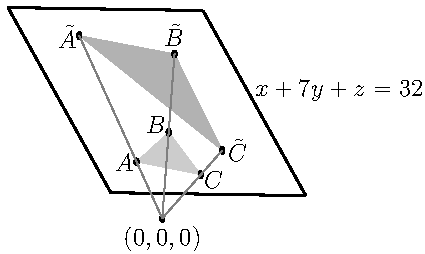
\includegraphics{OE16D_1.pdf}
\end{center}


\end{enumerate}
\end{question}

\begin{hint}
All three of the points $A$, $B$, $C$ lie in the plane $y=2$.
\end{hint}

\begin{answer}
(a) $x=0,\ y=2+t,\ z=2$\qquad
(b) The sphere $(x-1)^2 +(y-2)^2+(z-2)^2 = 1$

(c) $(0,4,4)$
\end{answer}

\begin{solution}
(a) We are given one point on the line, so we just need a
direction vector. That direction vector has to be perpendicular to the 
triangle $ABC$.

The fast way to get a direction vector is to observe that all 
three points $A$, $B$ and $C$, and consequently the entire triangle $ABC$,
are contained in the plane $y=2$. A normal vector to that plane, and 
consequently a direction vector for the desired line, is $\hj$.

Here is another, more mechanical, way to get a direction vector.
The vector from $A$ to $B$ is $\llt 2-0\,,\,2-2\,,\,2-2\rgt= \llt 2,0,0\rgt$
and the vector from $A$ to $C$ is $\llt 5-0\,,\,2-2\,,\,1-2\rgt= 
\llt 5,0,-1\rgt$. So a vector perpendicular to the triangle $ABC$ is
\begin{align*}
\llt 2,0,0\rgt \times \llt 5,0,-1\rgt
=\det\left[\begin{matrix}
            \hi  &  \hj  &  \hk \\
            2    &   0   &    0 \\
            5    &   0   &   -1 
            \end{matrix}\right]
=\llt 0 \,,\, 2 \,,\, 0 \rgt
\end{align*}
The vector $\frac{1}{2}\llt 0 \,,\, 2 \,,\, 0 \rgt=\llt 0 \,,\, 1 \,,\, 0 \rgt$
is also perpendicular to the triangle $ABC$. 

So the specified line has to contain the point $(0,2,2)$ and have direction
vector $\llt 0 , 1 , 0 \rgt$. The parametric equations
\begin{align*}
\llt x,y,z \rgt = \llt 0 , 2 , 2 \rgt + t\llt 0 , 1 , 0 \rgt
\end{align*}
or
\begin{align*}
x=0,\ 
y=2+t,\ 
z=2
\end{align*}
do the job.


\goodbreak
(b) Let $P$ be the point $(x,y,z)$. Then the vector from  $P$ to $A$
is $\llt 0-x\,,\,2-y\,,\,2-z\rgt$ and the vector from  $P$ to $B$
is $\llt 2-x\,,\,2-y\,,\,2-z\rgt$. These two vector are perpendicular
if and only if
\begin{align*}
0 &= \llt -x\,,\,2-y\,,\,2-z\rgt \cdot \llt 2-x\,,\,2-y\,,\,2-z\rgt
  = x(x-2) +(y-2)^2 +(z-2)^2 \\
  &= (x-1)^2 -1 +(y-2)^2 +(z-2)^2 
\end{align*}
This is a sphere.

(c) 
The light ray that forms $\tilde A$ starts at the origin,
passes through $A$ and then intersects the plane $x+7y+z=32$
at $\tilde A$. The line from the origin through $A$ has vector
parametric equation
\begin{align*}
\llt x,y,z\rgt = \llt 0,0,0 \rgt +t \llt 0,2,2\rgt
               =\llt 0,2t,2t\rgt
\end{align*}
This line intersects the plane $x+7y+z=32$ at the point whose value of $t$
obeys
\begin{align*}
(0) +7\overbrace{(2t)}^{y} +\overbrace{(2t)}^{z} =32
\iff t=2
\end{align*}
So $\tilde A$ is $(0,4,4)$.
\end{solution}

%%%%%%%%%%%%%%%%%%%%%%%%%%%%%%%%
\begin{question}
Let $P,\ Q,\ R$ and $S$ be the vertices of a tetrahedron.
Denote by $\vp,\ \vq,\ \vr$ and $\vs$ the vectors from the origin
to $P,\ Q,\ R$ and $S$ respectively. A line is drawn from each vertex to
the centroid of the opposite face, where the centroid of a triangle with 
vertices $\va,\ \vb$ and $\vc$ is $\frac{1}{3}(\va+\vb+\vc)$. 
Show that these four lines meet at $\frac{1}{4}(\vp+\vq+\vr+\vs$).
\end{question}

%\begin{hint}
%
%\end{hint}

\begin{answer}
See the solution.
\end{answer}

\begin{solution}
The face opposite $\vp$ is the triangle with vertices $\vq$, $\vr$ and $\vs$. 
The centroid of this triangle is $\frac{1}{3}(\vq+\vr+\vs)$. 
The direction vector of the line through $\vp$ and the 
centroid $\frac{1}{3}(\vq+\vr+\vs)$ is 
$\frac{1}{3}(\vq+\vr+\vs)-\vp$. The points on the line through
$\vp$ and the centroid $\frac{1}{3}(\vq+\vr+\vs)$ are those
of the form
\begin{equation*}
\vx=\vp+ t\left[\frac{1}{3}(\vq+\vr+\vs)-\vp\right]
\end{equation*}
for some real number $t$. Observe that when $t=\frac{3}{4}$
$$
\vp+ t\left[\frac{1}{3}(\vq+\vr+\vs)-\vp\right]
=\frac{1}{4}(\vp+\vq+\vr+\vs)
$$
so that $\frac{1}{4}(\vp+\vq+\vr+\vs)$ is on the line.
The other three lines have vector parametric equations
\begin{align*}
\vx&=\vq+ t\left[\frac{1}{3}(\vp+\vr+\vs)-\vq\right] \\
\vx&=\vr+ t\left[\frac{1}{3}(\vp+\vq+\vs)-\vr\right] \\
\vx&=\vs+ t\left[\frac{1}{3}(\vp+\vq+\vr)-\vs\right]
\end{align*}
When $t=\frac{3}{4}$, each of the three right hand sides also reduces
to $\frac{1}{4}(\vp+\vq+\vr+\vs)$ so that
$\frac{1}{4}(\vp+\vq+\vr+\vs)$ is also on each of these
three lines.
\end{solution}


%%%%%%%%%%%%%%%%%%%%%%%%%%%%%%%%
\begin{question}
Calculate the distance between the lines 
$\frac{x+2}{3}=\frac{y-7}{-4}=\frac{z-2}{4}$ and $\frac{x-1}{-3}=\frac{y+2}{4}=\frac{z+1}{1}$.
\end{question}

\begin{hint}
Review Example \eref{CLP200}{eg:VPdistance-line-line-bis}
in the CLP-3 text.
\end{hint}

\begin{answer}
$3$
\end{answer}

\begin{solution}
We'll use the procedure of Example \eref{CLP200}{eg:VPdistance-line-line-bis}
in the CLP-3 text. 
The vector 
\begin{equation*}
\llt 3,-4,4\rgt \times\llt -3,4,1\rgt 
=\det\left[\begin{matrix}
           \hi & \hj & \hk \\
           3  &  -4  &  4 \\
          -3  &   4  & 1
  \end{matrix}\right]
=\llt -20,-15,0\rgt 
\end{equation*}
is perpendicular to both lines. Hence so is 
$\vn=-\frac{1}{5}\llt -20,-15,0\rgt =\llt 4,3,0\rgt $. The point
$(-2,7,2)$ is on the first line and the point $(1,-2,-1)$ is on the second
line. Hence 
$\vv=\llt -2,7,2 \rgt-\llt1,-2,-1 \rgt=\llt -3,9,3\rgt $ is a vector 
joining the two lines. 
The desired distance is the length of the projection of $\vv$ on $\vn$. 
This is 
\begin{equation*}
\big|{\rm proj}_{\vn}\vv\big|
=\frac{|\llt -3,9,3\rgt \cdot\llt 4,3,0\rgt|}{|\llt 4,3,0\rgt|} 
=\frac{15}{5}=3
\end{equation*}
\end{solution}


